%% V1.3
%% 2007/01/11
%% by Michael Shell
%% see http://www.michaelshell.org/
%% for current contact information.
%%
%% This is a skeleton file demonstrating the use of IEEEtran.cls
%% (requires IEEEtran.cls version 1.7 or later) with an IEEE journal paper.
%%
%% Support sites:
%% http://www.michaelshell.org/tex/ieeetran/
%% http://www.ctan.org/tex-archive/macros/latex/contrib/IEEEtran/
%% and
%% http://www.ieee.org/



% *** Authors should verify (and, if needed, correct) their LaTeX system  ***
% *** with the testflow diagnostic prior to trusting their LaTeX platform ***
% *** with production work. IEEE's font choices can trigger bugs that do  ***
% *** not appear when using other class files.                            ***
% The testflow support page is at:
% http://www.michaelshell.org/tex/testflow/


%%*************************************************************************
%% Legal Notice:
%% This code is offered as-is without any warranty either expressed or
%% implied; without even the implied warranty of MERCHANTABILITY or
%% FITNESS FOR A PARTICULAR PURPOSE! 
%% User assumes all risk.
%% In no event shall IEEE or any contributor to this code be liable for
%% any damages or losses, including, but not limited to, incidental,
%% consequential, or any other damages, resulting from the use or misuse
%% of any information contained here.
%%
%% All comments are the opinions of their respective authors and are not
%% necessarily endorsed by the IEEE.
%%
%% This work is distributed under the LaTeX Project Public License (LPPL)
%% ( http://www.latex-project.org/ ) version 1.3, and may be freely used,
%% distributed and modified. A copy of the LPPL, version 1.3, is included
%% in the base LaTeX documentation of all distributions of LaTeX released
%% 2003/12/01 or later.
%% Retain all contribution notices and credits.
%% ** Modified files should be clearly indicated as such, including  **
%% ** renaming them and changing author support contact information. **
%%
%% File list of work: IEEEtran.cls, IEEEtran_HOWTO.pdf, bare_adv.tex,
%%                    bare_conf.tex, bare_jrnl.tex, bare_jrnl_compsoc.tex
%%*************************************************************************

% Note that the a4paper option is mainly intended so that authors in
% countries using A4 can easily print to A4 and see how their papers will
% look in print - the typesetting of the document will not typically be
% affected with changes in paper size (but the bottom and side margins will).
% Use the testflow package mentioned above to verify correct handling of
% both paper sizes by the user's LaTeX system.
%
% Also note that the "draftcls" or "draftclsnofoot", not "draft", option
% should be used if it is desired that the figures are to be displayed in
% draft mode.
%
\documentclass[journal, ]{IEEEtran}
\usepackage{cite}
\usepackage[pdftex]{graphicx}
\usepackage[cmex10]{amsmath}
% Also, note that the amsmath package sets \interdisplaylinepenalty to 10000
% thus preventing page breaks from occurring within multiline equations. Use:
%\interdisplaylinepenalty=2500
\usepackage{algorithmic}
\usepackage{array}
\usepackage{mdwmath}
\usepackage{mdwtab}
\usepackage{eqparbox}
%\usepackage[tight,footnotesize]{subfigure}
%\usepackage[caption=false]{caption}
\usepackage[font=footnotesize]{subfig}
\usepackage{fixltx2e}
\usepackage{stfloats}

\ifCLASSOPTIONcaptionsoff
  \usepackage[nomarkers]{endfloat}
  \let\MYoriglatexcaption\caption
  \renewcommand{\caption}[2][\relax]{\MYoriglatexcaption[#2]{#2}}
\fi
\usepackage{url}

% *** Do not adjust lengths that control margins, column widths, etc. ***
% *** Do not use packages that alter fonts (such as pslatex).         ***

% correct bad hyphenation here
\hyphenation{op-tical net-works semi-conduc-tor}

\usepackage{etoolbox}
\begin{document}
\title{Real or Not? NLP with Disaster Tweets EDA}

% author names and IEEE memberships
% note positions of commas and nonbreaking spaces ( ~ ) LaTeX will not break
% a structure at a ~ so this keeps an author's name from being broken across
% two lines.
% use \thanks{} to gain access to the first footnote area
% a separate \thanks must be used for each paragraph as LaTeX2e's \thanks
% was not built to handle multiple paragraphs
\author{Vegar~Andreas~Bergum,~\IEEEmembership{vab1g19,}
        ChangKai~Fu,~\IEEEmembership{ckf1n19,}
        Adam~Ghoumrassi,~\IEEEmembership{ag3u19,}
        PingChun~Tsai,~\IEEEmembership{pct1g19.}}
\markboth{COMP6208 Advanced Machine Learning}{}

% Reduces spacing between authors and text
\makeatletter
\patchcmd{\@maketitle}
  {\addvspace{0.5\baselineskip}\egroup}
  {\addvspace{-1.2\baselineskip}\egroup}
  {}
  {}
\makeatother

\maketitle

\begin{abstract}
This exploratory data analysis of the \textit{Real or Not? NLP with
Disaster Tweets} Kaggle competition dataset looks at possible underlying
patterns in the textual data contained in tweets. The analysis includes
syntactical features such as punctuation, spelling mistakes and word
frequencies, and semantic features such as sentiment, emojis and bigrams.
Further, we look at the top splits in a decision tree and perform latent
semantic analysis in an attempt to uncover lower-dimensional patterns. The
analysis reveals some underlying differences between the classes and
demonstrates how machine learning can be used on this classification problem.
\end{abstract}%

\IEEEpeerreviewmaketitle

% needed in second column of first page if using \IEEEpubid
%\IEEEpubidadjcol

\section{Introduction}
\IEEEPARstart{T}{his} project considers the \textit{Real or Not? NLP
with Disaster
Tweets}\footnote{\url{https://www.kaggle.com/c/nlp-getting-started/overview}}
Kaggle competition, where one attempts to classify whether or not a tweet is
announcing a real disaster. As stated in the competition; ''Twitter has become
an important communication channel in times of emergency``, both by government
organisations and individuals. With this comes the challenge of fake news and
the general authenticity of the information being spread online. With the
capability of quickly and reliably classifying any given tweet as announcing a
real disaster or not, one can help improve automatic disaster monitoring.\\

With any machine learning project, one of the most important steps is exploring
the data available. In this competition, we have access to $7,613$ labelled
tweets (fake and real). Most of this data is pure text (the content of the
tweets), which makes this a natural language processing (NLP) task. Feature
extraction is very important and complex when working with textual natural
language. There are several methods for representing the semantics of text,
including word-frequency based approaches such as TF-IDF and more advanced
latent space representations such as word embeddings like
\textit{word2vec}\cite{mikolov2013}. In order to get a better understanding of
the existing features in the data and basis for choosing a semantic
representation model, we explore both token- and character-level relationships
between the data and the two classes.

\section{Data Summarization}
The data set contains $7,613$ tweets, labelled as fake and real. Excluding the
label, the data has three main attributes: \textit{keyword, location, text}.
The keyword attribute contains a list of pre-defined keywords that describes
the contents of the tweet. The location is provided directly by Twitter's
geo-tag on a tweet and is represented as a string, e.g. \textit{New York
City}. The text attribute holds the vast majority of the data, as this is the
raw textual content of the tweet. Table \ref{tab:missing_values} shows the
percentage of missing values and unique entries in each attribute. 

\begin{table}[hbt!]
  \begin{center}
  \begin{tabular}{c|c|c} 
   \hline
    \textbf{Attribute} & \textbf{Missing values}  & \textbf{Unique entries}\\
    keyword & 0.8\% & 61\\
    location & 33.3\% & 2,533\\
    text & 0.0\% & 7,613\\
   \hline
  \end{tabular}
  \end{center}
  \caption{Missing and unique values in the data attributes.}
  \label{tab:missing_values}
\end{table}

As can be seen from the table, a third of the location data is missing. The
keyword attribute is only missing a relatively few number of entries, although
it should be noted that the number of unique keywords is quite low. Further,
Figure \ref{fig:class_proportions} shows the proportions of tweets in both
classes. There is a slight unbalance in the dataset, however, this is
considered low enough to not have any substantial effects on the problem
modeling.

\begin{figure}[hbt!]
  \centering
  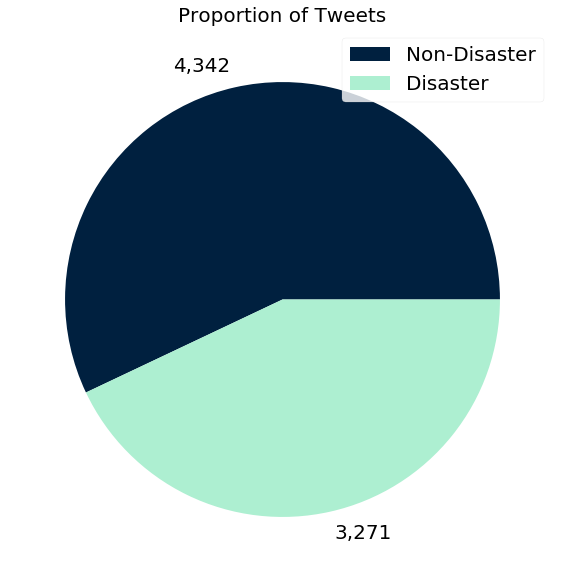
\includegraphics[width=0.7\linewidth]{../figures/class_proportion.png}
  \caption{Class proportions.}
  \label{fig:class_proportions}
\end{figure}

\section{Quantitative Statistics}
Exploring the textual data in the corpus reveals some correlations between the
various syntactic and semantic features, and the two classes. Figure
\ref{fig:num_words} shows that there is a small shift in the mean of the
average number of words per tweet between the two classes. Non-disaster (fake)
tweets are, on average, shorter and have a larger variation in tweet size. This
implies that the tweet length could be a useful feature for classification.\\

\begin{figure}[hbt!]
  \centering
  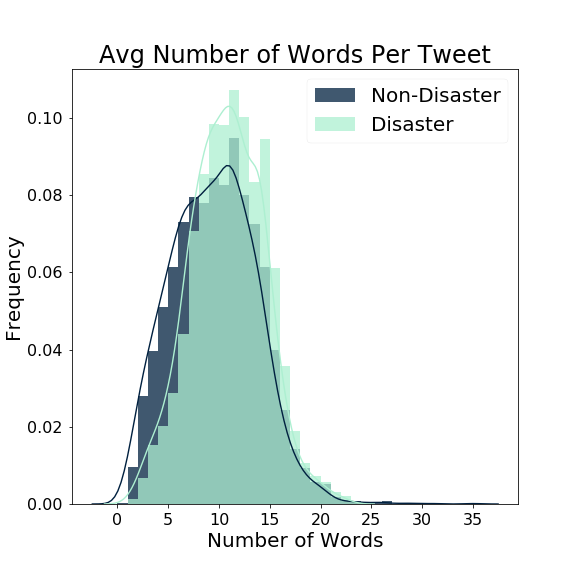
\includegraphics[width=0.7\linewidth]{../figures/num_words.png}
  \caption{Distribution of average number of words per tweet.}
  \label{fig:num_words}
\end{figure}

Emojis have a prominent presence in social media, also on Twitter.
Unfortunately, the text in the dataset is encoded in such a way that emojis can
not be distinguished from each other. However, one can still look at the
frequency of their use. \textit{A priori} one could argue that a real disaster tweet
is often from a mainstream news source and would stray away from using informal
language and symbols, such as emojis. Figure \ref{fig:emoji_freq}, showing the
frequency of emoji-usage, confirms this hypothesis. Non-disaster tweets use
emojis more regularly than real disaster tweets. Since emojis are encoded as a
special escape-sequence they can be considered as a semantic token equivalently
to a regular word when modeling the problem for classification.

\begin{figure}[hbt!]
  \centering
  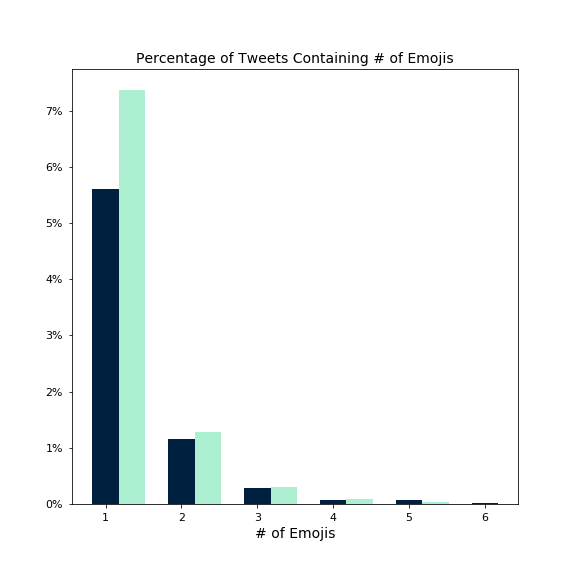
\includegraphics[width=0.7\linewidth]{../figures/emoji_freq.png}
  \caption{Frequency of emoji-usage in the two classes.}
  \label{fig:emoji_freq}
\end{figure}

The use of external links has shown to be a large differentiator between the
two classes. 50\% of non-disaster tweets contain external links, compared to
78\% of disaster tweets. A rationale for this difference is that disaster
tweets often refer to a source or proof of the disaster. Looking into the links
being used, we can observe a difference in pages that are linked to from the
two classes. Figure \ref{fig:domain_freq} shows the top 15 referred-to domains
by the two classes. Observe that the disaster tweets are linking to official
news sites such as \texttt{bbc.co.uk}, \texttt{latimes.com}, \texttt{cnn.com},
while the non-disaster tweets link to other social-medias sites such as
\texttt{facebook.com} and \texttt{instagram.com}, \texttt{ebay.com} and various
blogs. 

\begin{figure}[hbt!]
  \centering
  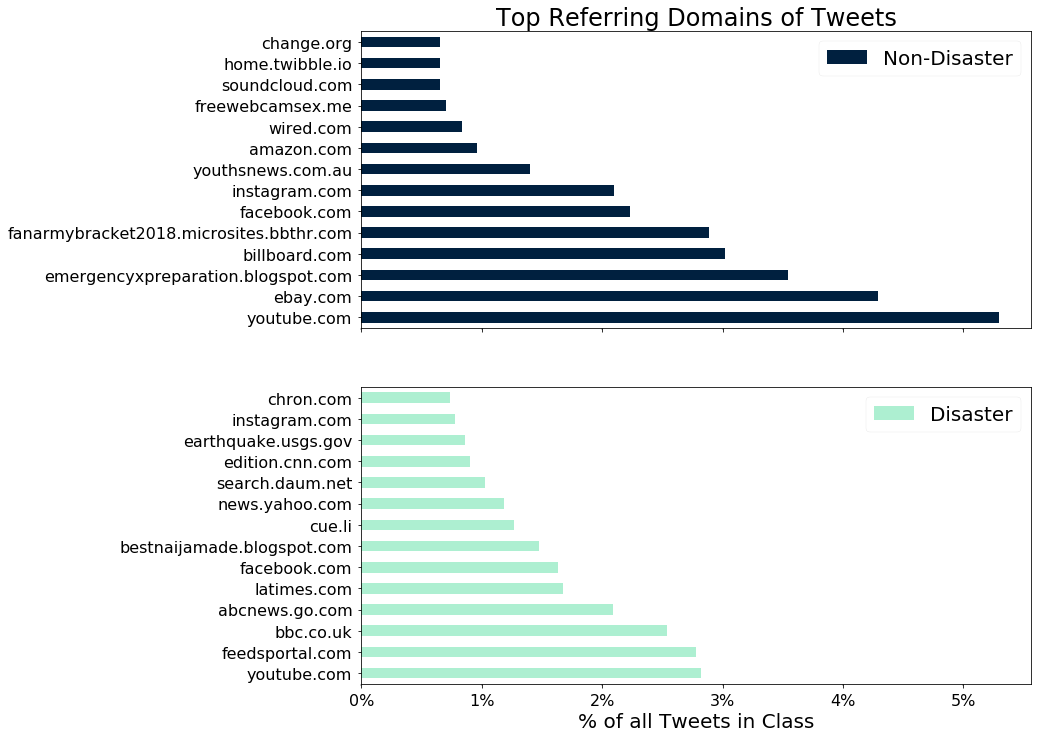
\includegraphics[width=\linewidth]{../figures/domain_freq.png}
  \caption{Top domains for links in tweets.}
  \label{fig:domain_freq}
\end{figure}

When considering the use of punctuation in the tweet texts we observe a few
differences between the two classes. Symbols such as \texttt{\{} and \texttt{$>$}
appear exclusively in the non-disaster tweets, although at a very low
frequency. Other symbols such as \texttt{=, /\, and `} also vary largely
between the two classes. By manual inspection of the tweets that account for
these differences there are no obvious reason for the large difference. Since
the highest varying punctuation symbols also are the least used symbols, we
assume that the large variation is simply due to the sampling bias of such a
low frequency of their use. 
\begin{figure}[hbt!]
  \centering
  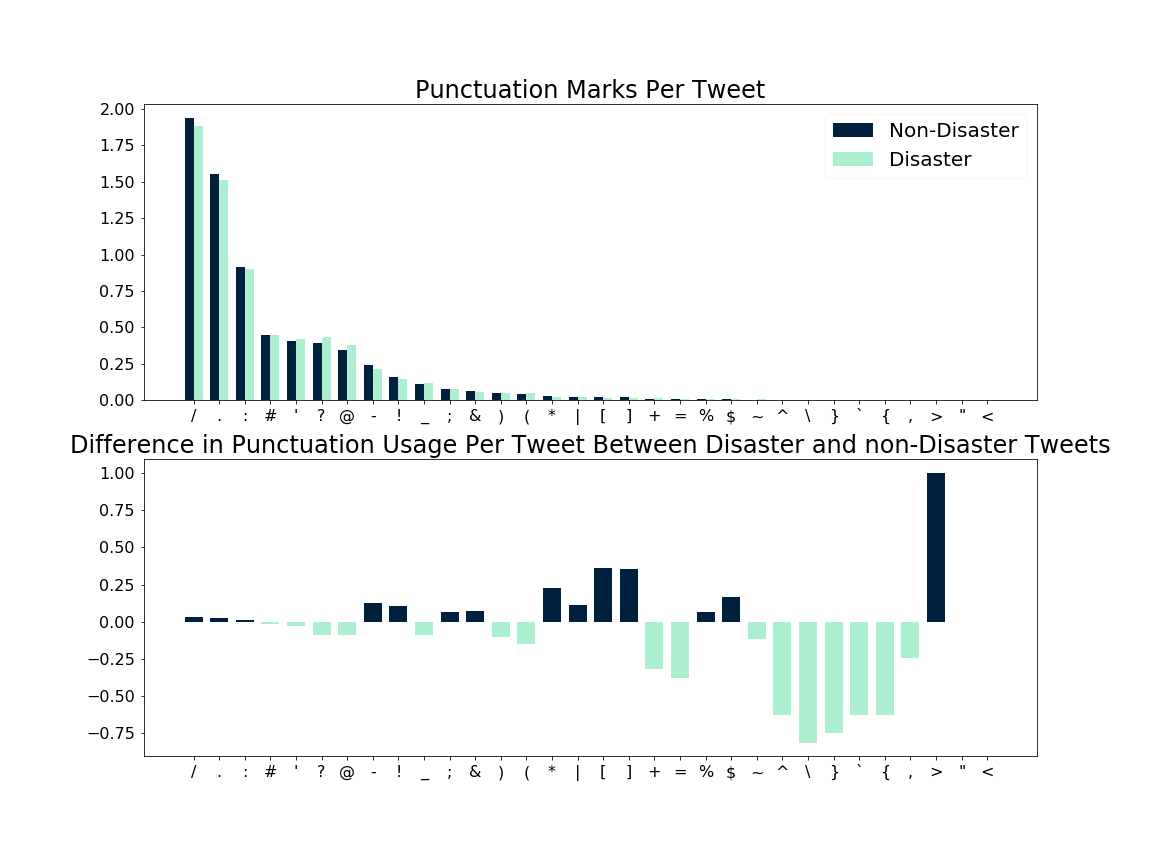
\includegraphics[width=\linewidth]{../figures/punctuation.png}
  \caption{Use of punctuation per tweet and differences in use between classes.}
  \label{fig:punctuation}
\end{figure}

Figure \ref{fig:part_of_speech} illustrates some of the different linguistic
features of the two classes by showing the distribution and difference in
part-of-speech tags per tweet. Notably, the disaster tweets more often use
numbers and proper nouns. One explanation of this difference would be the
larger amount of references to statistics (numbers) and official bodies and
names (proper nouns) in real disaster coverage. However, the difference is very
minimal for all POS-tags, so this could simply be an arbitrary difference due
to noise. The \texttt{en\_core\_web\_sm} POS-tagger in \texttt{spacy} was used for
tagging.

\begin{figure}[hbt!]
  \centering
  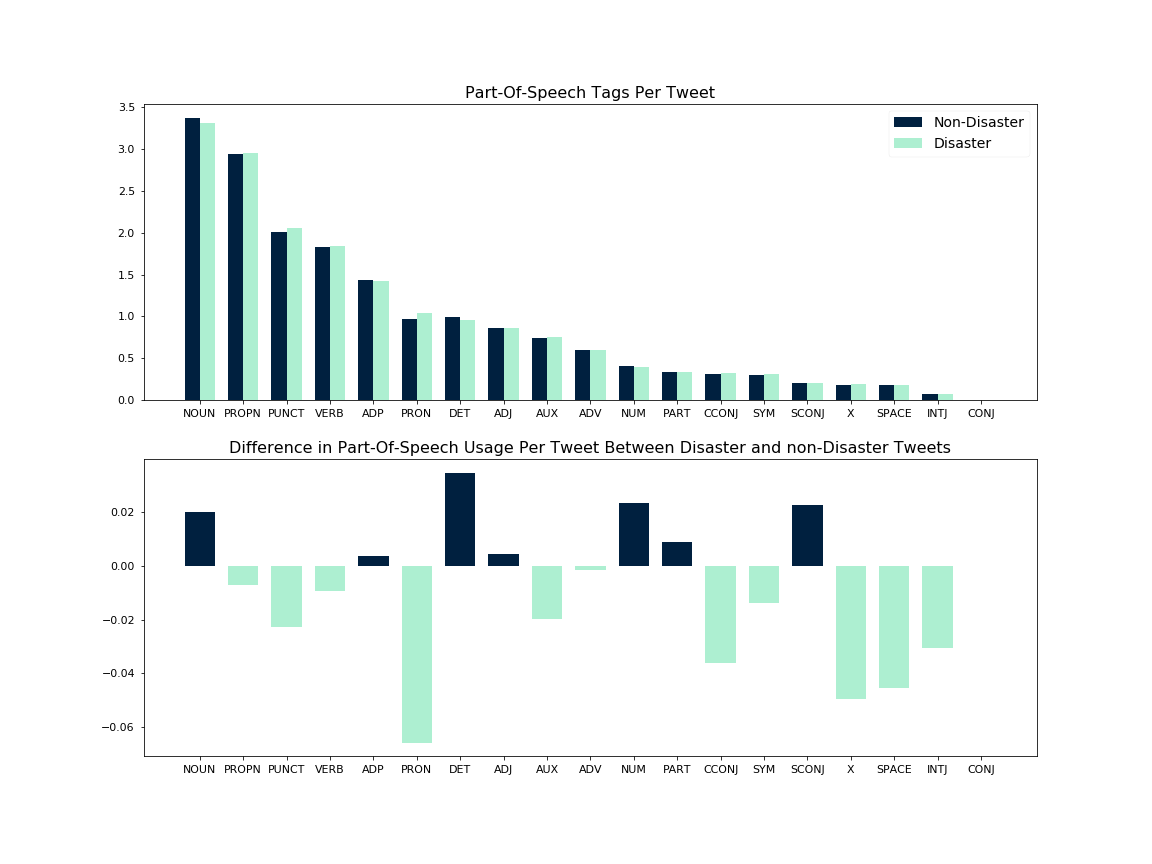
\includegraphics[width=\linewidth]{../figures/part_of_speech.png}
  \caption{Distribution of POS tags per tweet and differences between classes.}
  \label{fig:part_of_speech}
\end{figure}

Using a Hamilton distance of 1 between two tokens and the WordFrequency
project\footnote{https://github.com/hermitdave/FrequencyWords} dictionary to
correct spelling, we evaluate the number of spelling mistakes per tweet, per
class. Figure \ref{fig:spelling_mistakes} shows the number of spelling
mistakes for both classes. We observe that except for tweets with a single
spelling mistake, disaster tweets contain more mistakes than non-disaster
tweets. These differences are very small and lay within the margin of error to
be expected from this approach to detecting spelling mistakes.

\begin{figure}[hbt!]
  \centering
  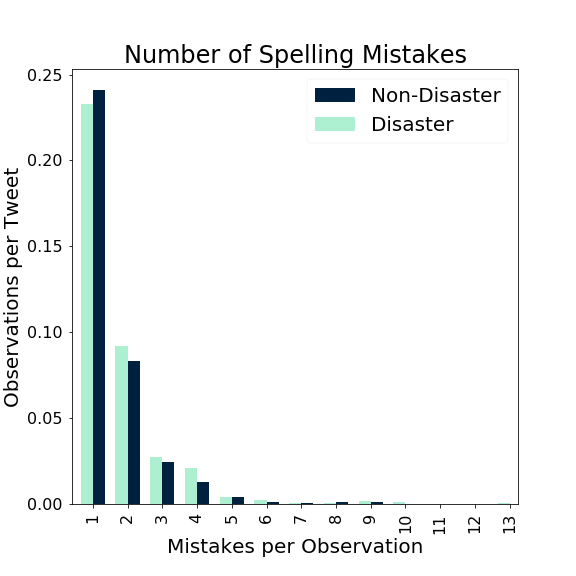
\includegraphics[width=0.9\linewidth]{../figures/spelling_mistakes.png}
  \caption{Frequency of spelling mistakes per tweet.}
  \label{fig:spelling_mistakes}
\end{figure}

\section{Sentiment analysis}
As we have seen from the investigation into the use of external links, many of
the real disaster tweets are referring to large mainstream news sources. News
is supposed to be objective and carry little to no sentiment. Using VADER
Sentiment Analysis\footnote{\url{https://github.com/cjhutto/vaderSentiment}}, a
rule-based sentiment analysis tool that is specifically made for social media
text, we investigate the correlation between sentiment and subjectivity, and
classes. Figure \ref{fig:sent_sub_dist} shows a distribution and density of
sentiment and subjectivity scores. Note that the two classes are laid on top of
each other in both figures. A negative sentiment value naturally corresponds to
negative sentiment, positive values correspond to positive sentiment and 0
corresponds to a neutral or non-sentimental tweet. A subjectivity score of 0
corresponds to an objective text, where 1 corresponds to maximum subjectivity.

\begin{figure}[hbt!]
  \centering
  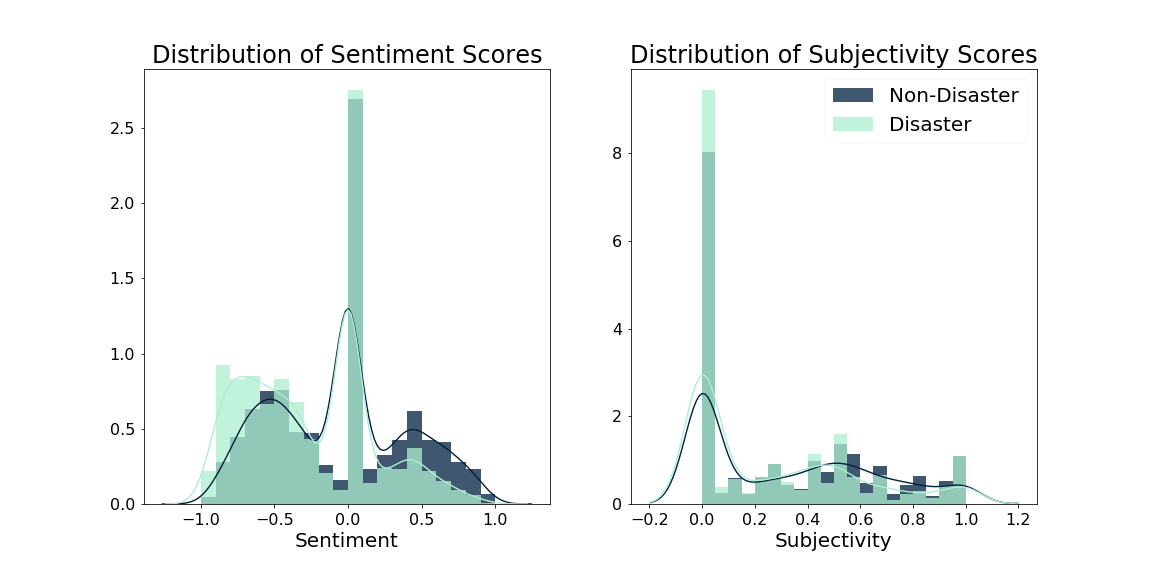
\includegraphics[width=\linewidth]{../figures/sent_sub_dist.png}
  \caption{Distribution and sentiment }
  \label{fig:sent_sub_dist}
\end{figure}

Observe that disaster tweets are more frequently objective and neutral.
Additionally, non-disaster tweets carry more positive sentiment while disaster
tweets are negative more often. Non-disaster tweets are also slightly skewed
towards being more subjective than real disaster tweets. These observations all
follow the intuition of disaster tweets being either mostly neutral and
objective (reported news) or carry a negative sentiment. 

\begin{table}[hbt!]
  \begin{center}
   \begin{tabular}{c|c|c|c|c} 
   \hline
    \textbf{Class} & \textbf{Negative} & 
      \textbf{Neutral} & \textbf{Positive} & \textbf{Subjective}\\
    Non-Disaster & 0.132 & 0.766 & 0.102 & 0.324\\
    Disaster & 0.173 & 0.777 & 0.049 & 0.265\\
   \hline
  \end{tabular}
  \end{center}
  \caption{Mean values of negative, neutral and positive sentiment as well as
  mean subjectivity of tweets for each class.}
  \label{tab:sentiment}
\end{table}

Table \ref{tab:sentiment} shows the mean values of sentiment and
subjectivity for the two classes. These values further quantifies the
differences. Disaster tweets are 20\% more objective, 71\% less positive
and 27\% more negative than non-disaster tweets. 

\section{Feature Exploration}
% TF-IDF + cosine, D-tree vis, PCA, n-grams, Non-ML modeling.
To explore some of the most prominent textual and semantic features in the
dataset, we consider a few models that are suitable for extracting said
features. Figure \ref{fig:decision_tree} shows the first few nodes in a
decision tree trained based on word frequency. The tree classifies the tweets
with an F1-score of $0.76$. Notably, from the top of the tree we observe that
words such as \textit{suicide, California, killed, ISIS, bomb} and
\textit{west} are immediately recognised as features contributing to a good
split. These are also tokens that one would consider as substantial in
differentiation between a disaster and non-disaster tweet. This shows that the
data contains useful features for class separation.

\begin{figure}[hbt!]
  \centering
  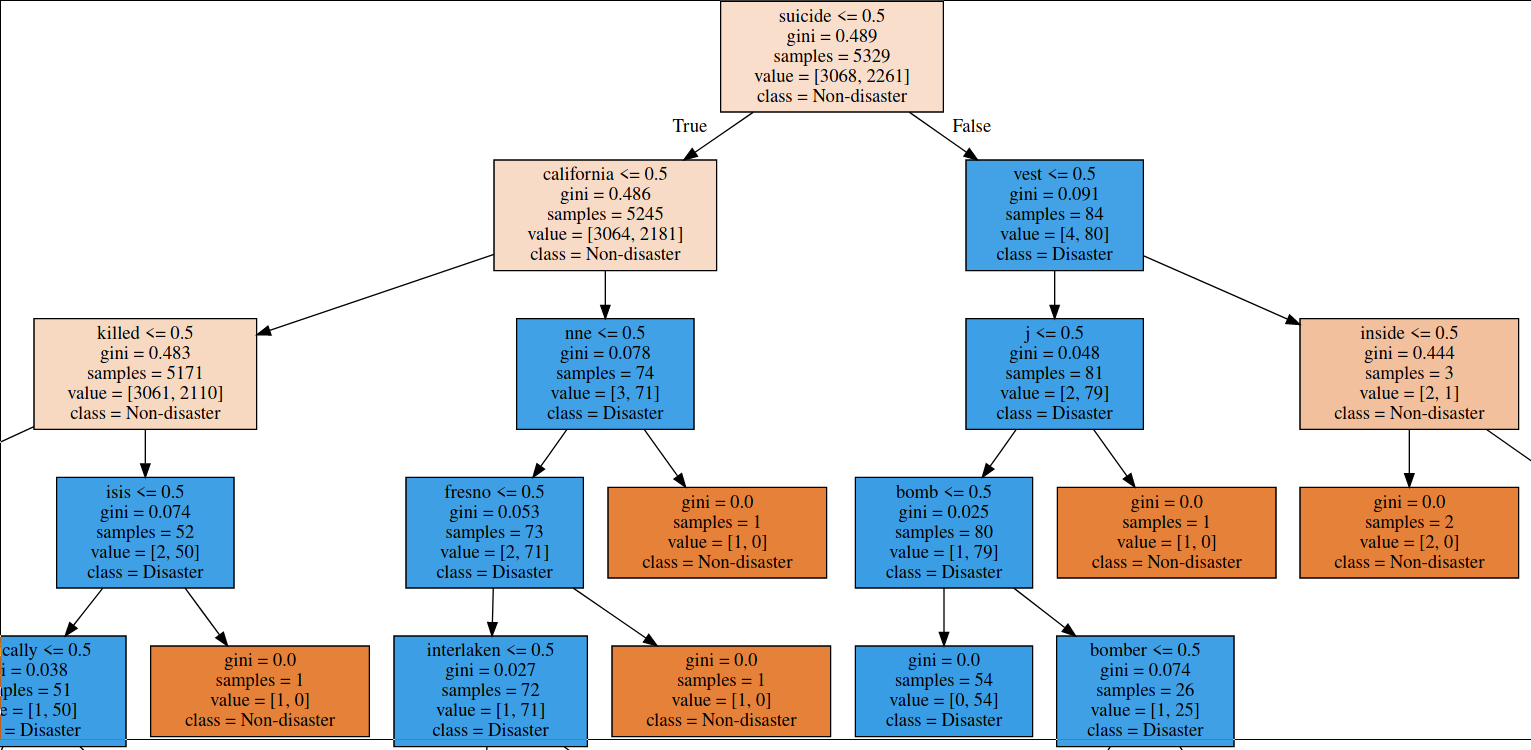
\includegraphics[width=\linewidth]{../figures/decision_tree.png}
  \caption{First few nodes of a decision tree achieving an F1 score of 0.76.}
  \label{fig:decision_tree}
\end{figure}

However, the vocabulary size of the textual data is over 7000 unique words.
Data with such a high dimensionality can cause some problems when attempting
to extract useful features. Using PCA, we attempt to reduce the dimensionality
(substantially) and visualise the results to see if there are any evident
patterns, even at 2- and 3D. Figure \ref{fig:pca} shows a 2D PCA projection
of the textual data. Other than the slightly higher variation in the
non-disaster data, including a few outliers, there are no evident patterns that
helps separate the two classes. The same results are evident in the 3D
projection of the data. 

\begin{figure}[hbt!]
  \centering
  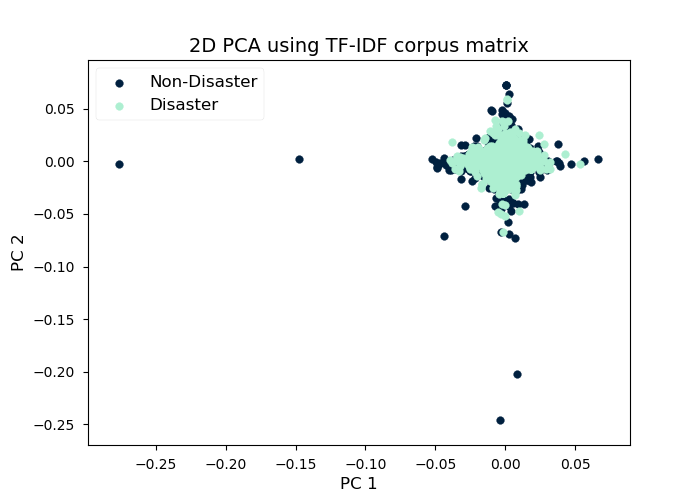
\includegraphics[width=\linewidth]{../figures/pca.png}
  \caption{2 dimensional PCA using a TF-IDF corpus matrix.}
  \label{fig:pca}
\end{figure}

From a probabilistic view, we can build a basic language model using the n-gram
model, specifically a 2-gram (bigram) model. Using this Markov chain model we
can investigate the most frequent bigrams from two models built on each data
class. Figure \ref{fig:ngram} shows the top 10 bigrams for both classes, which
illustrates some expected differences. Although the two classes share some
frequent bigrams such as \textit{burning building(s)}, the disaster model
mostly contains bigrams that are clearly related to disasters. While the
non-disaster language model contains what can be seen as more arbitrary bigrams
of words. The disaster tweets also have a clearer variation in the frequency of
its top 10 bigrams, where a few specific disasters are overrepresented, such as
the Malaysian airlines disaster.

\begin{figure}[hbt!]
  \centering
  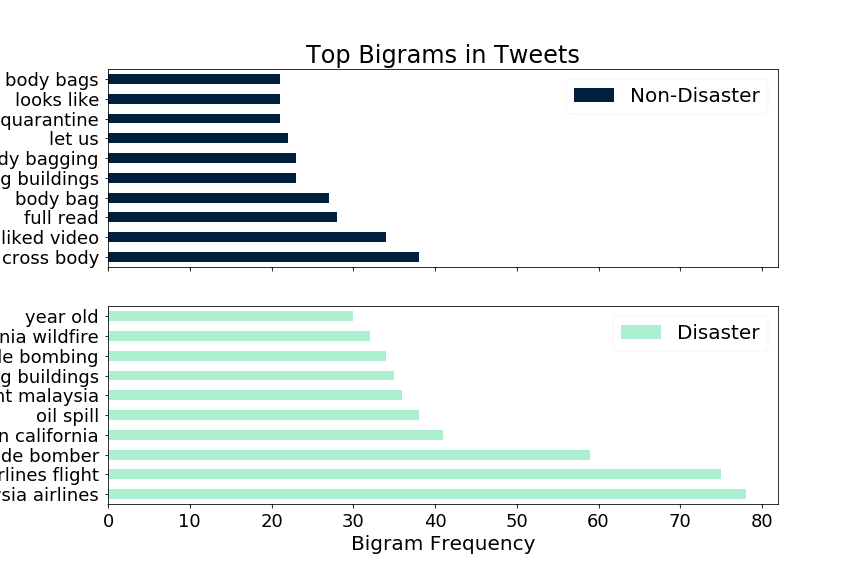
\includegraphics[width=\linewidth]{../figures/ngrams.png}
  \caption{Top 10 Bigrams.}
  \label{fig:ngram}
\end{figure}

\section{Conclusion}
In the data exploration part of this project, we analysed the data layer by
layer like peeling an onion. In the beginning, we utilized quantitative
statistics to generate the number of words per tweet, frequency of emoji-usage,
top (website) domains for links in tweets, use of punctuation, part-of-speech
tags and the frequency of spelling mistake to observe the differences between
the two classes using various characteristics and elements of the text.
Fortunately, we did observe some patterns worth mentioning between the two
classes. We observed that the tweets labelled as real tend to include less
emojis, link to official news sites, and the distribution of the average words
in disaster class shifts to larger number compared to non-disaster class. These
mentioned patterns interested us to investigate the sentiment of the tweeters
as real disaster tweets are more likely to be originated from news or a
serious/negative emotion. Thus, the distribution of sentiment and subjectivity
scores of tweets were analysed to see if we could have a clearer insight.

However, the results are still not obvious enough to differentiate the disaster
and non-disaster classes as tweets data are very noisy. Therefore, we tried to
extract the prominent features by using TF-IDF and a decision tree. The vectors
processed by TF-IDF and PCA seems to have no clear evidence to classify the two
classes as it is the standard way of performing a latent semantic analysis
(LSA). In comparison, the decision tree model achieved an F1-score of 0.76,
which is a good result and the power of machine learning is uncovered. In the
next stage of the project, we will be using word embedding method such as
word2vec, BERT and sequence-to-sequence RNN to find out the patterns between
tiny differences which are hard to be found by the existing methods.

% Can use something like this to put references on a page
% by themselves when using endfloat and the captionsoff option.
\ifCLASSOPTIONcaptionsoff
  \newpage
\fi

% trigger a \newpage just before the given reference
% number - used to balance the columns on the last page
% adjust value as needed - may need to be readjusted if
% the document is modified later
%\IEEEtriggeratref{8}
% The "triggered" command can be changed if desired:
%\IEEEtriggercmd{\enlargethispage{-5in}}

% references section

% can use a bibliography generated by BibTeX as a .bbl file
% BibTeX documentation can be easily obtained at:
% http://www.ctan.org/tex-archive/biblio/bibtex/contrib/doc/
% The IEEEtran BibTeX style support page is at:
% http://www.michaelshell.org/tex/ieeetran/bibtex/
\bibliographystyle{IEEEtran}
% argument is your BibTeX string definitions and bibliography database(s)
%\bibliography{IEEEabrv,../bib/paper}
%
% <OR> manually copy in the resultant .bbl file
% set second argument of \begin to the number of references
% (used to reserve space for the reference number labels box)

\bibliography{references.bib}

\end{document}
